\documentclass[8pt, letterpaper, titlepage]{article}
\usepackage[utf8]{inputenc}
\usepackage{geometry}
\usepackage{color,graphicx,overpic} 
\usepackage{fancyhdr}
\usepackage{amsmath,amsthm,amsfonts,amssymb}
\usepackage{mathtools}
\usepackage{hyperref}
\usepackage{multicol}
\usepackage{array}
\usepackage{float}
\usepackage{blindtext}
\usepackage{longtable}
\usepackage{scrextend}
\usepackage[font=small,labelfont=bf]{caption}
\usepackage[framemethod=tikz]{mdframed}
\usepackage{calc}
\usepackage{titlesec}
\usepackage{listings}
\usepackage[normalem]{ulem}
\usepackage{tabularx}
\usepackage{mathrsfs}
\usepackage{bookmark}
\usepackage{setspace}
\usepackage{tabularx}
\usepackage{ltablex}
\usepackage{enumitem}
\usepackage[simplified]{pgf
-umlcd}

\mathtoolsset{showonlyrefs}  
\allowdisplaybreaks

\definecolor{mycolor}{rgb}{0, 0, 0}

\geometry{top=1cm, left=1cm, right=1cm, bottom=1cm}
\setlength{\headheight}{20pt}
\setlength{\parskip}{0.15cm}
\setlength{\parindent}{0cm}

\definecolor{dkgreen}{rgb}{0,0.6,0}
\definecolor{gray}{rgb}{0.5,0.5,0.5}
\definecolor{mauve}{rgb}{0.58,0,0.82}

\lstset{frame=tb,
  language=Java,
  aboveskip=3mm,
  belowskip=3mm,
  showstringspaces=false,
  columns=flexible,
  basicstyle={\small\ttfamily},
  numbers=none,
  numberstyle=\tiny\color{gray},
  keywordstyle=\color{blue},
  commentstyle=\color{dkgreen},
  stringstyle=\color{mauve},
  breaklines=true,
  breakatwhitespace=true,
  tabsize=3
}

\begin{document}
\begin{multicols*}{2}
\footnotesize
\subsection*{Objects, UML, and Java}
\textbf{Abstraction:} Simplifying to its essentials the description of a real-world entity or concept.

\textbf{Encapsulation:} Building data with access functions distinguishing ``what'' from ``how.''

\textbf{Decomposition:} Dividing whole things into parts or composing whole things out of parts.

\textbf{Generalization:} From specific cases, looking for commonalities that can be factored out.

\textbf{Abstract Class v.s. Interface:} An abstract class may provide a partial implementation. A class may implement any number of interfaces, but only extend one superclass. Adding a method to an interface will ``break'' any class that  previously implemented it.

\textbf{Java Subtleties}
\begin{lstlisting}[basicstyle=\footnotesize\ttfamily]
// Constructor super call
public class Base {
    protected int value;
    public Base( int initValue ) {
        // implicitly inserted call to super()
        value = initValue;
    }
}
public class Derived extends Base {
    public Derived( int initValue ) {
        super( initValue );
        // explicit call to super();
        // super() if used, must come first
    }
}

// Shadowing data
public class Base {
    protected int value; // 2, 3
}
public class Derived extends Base {
    private int value; // 0, 1
    public void test() {
        value = 0;
        this.value = 1;
        super.value = 2;
        ((Base)this).value = 3;
    }
} 

// Overriding is not Shadowing
public class Base {
    public int i = 1;
    public int f() { return i; }
}
public class Derived extends Base {
    public int i = 2; // shadowing
    public int f() { return -i; } // overriding
}
public class Test {
    public static void main( String args[] ) {
        Derived d = new Derived();
        // d.i is 2, d.f() returns -2
        Base b = (Base)d;
        // b.i is 1, b.f() returns -2, "dynamic binding"
    }
}
\end{lstlisting}

\textbf{CRC Cards}
Class-Responsibility-Collaborator: Explore classes, their responsibilities, and their interactions.
\begin{figure}[H]
    \centering
    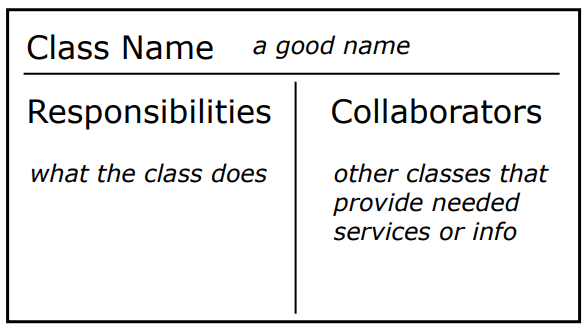
\includegraphics[width=0.2\textwidth]{CRC.png}
\end{figure}

\subsection*{Software Process}

\textbf{Waterfall:}
\begin{figure}[H]
    \centering
    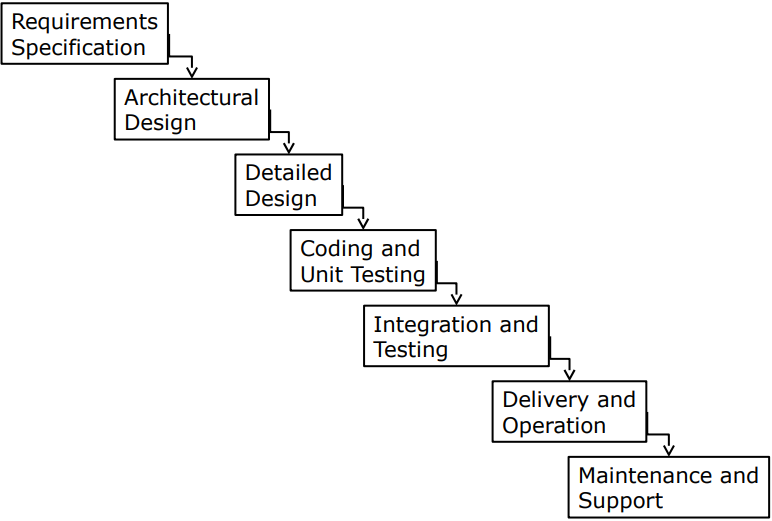
\includegraphics[width=0.23\textwidth]{Waterfall.png}
\end{figure}
\begin{itemize}
    \item Pros: easily understood, enforces discipline, verification at every phase, documentation
    \item Cons: uses a manufacturing view of software, customer must be patient, customer sees the system only at the end, dependence on requirements being ``right,'' requirements must all be known up front
\end{itemize}

\textbf{Prototyping:} Making sure you develop the right system. Iterative design: cycling through several designs, improving the product with each pass. Various approaches: throwaway, incremental, evolutionary.
\begin{itemize}
    \item Throwaway: Build and test prototype, gain knowledge for the real product, ``throw away'' the prototype, then develop the ``product'' for real.
    \begin{itemize}
        \item Pros: more communication between users and developers, functionality introduced earlier which is good for morale
        \item Cons: building the prototype must be rapid, some qualities may be sacrificed, temptation to use the throwaway prototype in the final product
    \end{itemize}
    \item Incremental: Triage system into separate increments (i.e. ``must do'', ``should do'', ``could do''), develop and add one increment at a time.
    \item Evolutionary: feature is refined or ``evolved'' over time
    \item Other: user interface sketches, storyboards
\end{itemize}

\textbf{Staged delivery:} Developers deliver the system  in a series of working releases or builds. Users use some functionality while the rest continues to be developed. 
\begin{itemize}
    \item Pros: provides more options, different builds focus on specific features, reduces estimation errors, risks are reduced earlier.
    \item Cons: Overhead needed to plan and drive the product toward staged releases, extra complexity of supporting multiple versions in the field.
\end{itemize}

\textbf{Agile Practices:} trust motivated individuals, face-to-face conversation, best work emerges from self-organizing teams, team reflects on and adjusts their behavior, promote constant, sustainable pace. ``Working software'' is the main measure of progress. Continuous, frequent delivery of value. Customers and developers work together, satisfy customer early. Welcome changing requirements.
\begin{itemize}
    \item eXtreme Programming (XP): Communication, feedback, simplicity, programmer friendly (40h work week), code-centric, for small teams (up to about 20), and requires courage. 12 practices: 40 hour week, metaphor, simple design, collective ownership, coding standards, small releases, continuous integration, refactoring, planning game, testing, on-site customer, and pair programming.
    \item Scrum: Agile process, doesn't prescribe many development methods. Based around feedback, roles, meetings, prioritization, and planning. Scrum Master protects the team and helps the team follow scrum. Product owner represents the customer. Scrum meetings:
    \begin{itemize}
        \item Planning Meeting (take requirements and user stories. Choose appropriate stories to work on next, estimate their cost in time, prioritize them, and fit them into the time left for the iteration)
        \item Daily Scrum (time limited, every team member answers: what did they do, what are they going to do, and what they are blocked by.)
        \item Retrospective (review issues faced with quality and personnel, try to improve the process)
        \item Review (review work completed and not completed, demonstrate current system)
    \end{itemize}
\end{itemize}

\subsection*{Requirements}

Types:
\begin{itemize}
    \item User requirements (what tasks the user can do with the system)
    \item Functional requirements (features: what behaviors the system does or supports)
    \item Non-functional requirements (qualities: how well the system should do what it does, e.g., response time, resources usage)
\end{itemize}

SMART Work Items: Specific, Measurable, Achievable, Relevant, Time Boxed. INVEST in Good Stories: Independent, Negotiable, Valuable, Estimable, Small, Testable.

\subsection*{Testing}

Examples of Defects:
\begin{itemize}
    \item Algorithmic: code logic does not produce the proper output
    \item Overload: data structure unexpectedly filled to capacity
    \item Performance: violates service level agreement
    \item Accuracy: calculated result not to the desired level of accuracy
    \item Timing: race condition in coordinating concurrent processes
\end{itemize}

\textbf{Regression Testing:} Avoid breaking things that should work. Do regression test after a change or fix to check whether previously passing tests now fail.

\textbf{Black Box Testing:} Be systematic about what to test not knowing the internal code. Determine equivalence classes: each test inside an equivalence class checks the ``same thing''. 

\textbf{Testing Strategies:}
\begin{itemize}
    \item Big-bang strategy: test thoroughly only after the whole system is put together. Pro: project almost finished, only testing left. Con: hard to pinpoint cause of failure.
    \item Top-down incremental strategy: implement/test the highest-level modules first. Use stubs for lower-level functionality, higher-level modules are the test drivers.
    \item Bottom-up incremental strategy: implement/test the lowest-level modules first, need to write test drivers.
\end{itemize}

\textbf{Automated Testing:} Write software to help test software. Essential to test-driven development and refactoring.

\textbf{Test Driven Development:} Write tests first.

\textbf{JUnit Framework:}
Example test code:
\begin{lstlisting}[basicstyle=\footnotesize\ttfamily]
public class NumberTest extends TestCase {
    private Number aNumber;
    private Number anotherNumber;
    
    protected void setUp() {
        aNumber = new Number(2);
        anotherNumber = new Number(3);
    }
    // check that value-based equality works
    public void testEquals() {
        Assert.assertTrue(!aNumber.equals(null));
        Assert.assertEquals(aNumber, aNumber);
        Assert.assertEquals(aNumber, new Number(2));
        Assert.assertTrue(!aNumber.equals(anotherNumber));
    }
}
\end{lstlisting}
\begin{itemize}
    \item \lstinline{setUp()} method to initialize the test objects (or fixture) before each test method is run.
    \item \lstinline{tearDown()} method to clean up the fixture afterwards
\end{itemize}

\subsection*{Refactoring}

Change software system so that external behavior does not change but internal structure is improved. Do this in small steps (change a bit and re-test). When adding a feature, refactor to make the addition easier to achieve. 

\textbf{Code Smells:}
\begin{itemize}
    \item Duplicated Code: Extract Method, Pull Up Method
    \item Long Method (long, difficult-to-understand methods): Extract Method
    \item Large Class (Blob or God Class trying to do too many things): Extract Class
    \item Divergent Change (a class is commonly changed in different ways for different reasons): Extract Class
    \item Shotgun Surgery (making a change requires many little changes across many different classes or methods): Move Method
    \item Long Parameter List: Replace parameter with method, introduce parameter object
    \item Feature Envy (method seems more interested in details of a class other than the one it is in): Move Method, Extract Method 
    \item Data Class (class that is just data): Encapsulate Field, Extract Method, Move Method 
    \item Data Clumps (groups of data appearing together in the instance variables of classes, parameters to methods, etc.): Extract Class, Introduce Parameter Object 
    \item Primitive Obsession (using the built-in types too much): Replace Data Value with Object
    \item Switch Statements (long conditionals on type codes defined in other classes): Extract/Move Method, Replace Type Code, Replace Conditional with Polymorphism
    \item Speculative Generality (``we might need this someday''): Collapse Hierarchy, Remove Parameter
    \item Message Chains (long chains of navigation to get to an object): Hide Delegate
    \item Inappropriate Intimacy (two classes that depend too much on each other, with lots of bidirectional communication): Move Method, Extract Class 
    \item Refused Bequest (subclass inherits something that is not needed): Push Down Method and Push Down Field, Replace Inheritance with Delegation
\end{itemize}

\normalsize
\end{multicols*}

\newpage

\begin{multicols*}{3}
\textbf{UML Class Diagrams}

\begin{tikzpicture}
    \begin{class}[text width=5cm]{Classname}{0,0}
    \attribute{+ attribute : type}
    \operation{+ publicMethod() : type}
    % virtual operation
    \operation{- privateMethod() : type}
    \operation{\# protectedMethod() : type}
    \end{class}
\end {tikzpicture} \\
\textbf{Association}: Used when two models need to communicate between each other.
\begin{center}
    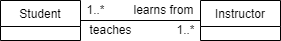
\includegraphics[width=4cm]{uni.png}
\end{center}
A student can have one or more instructors. An instructor can have one or more students.

\textbf{Aggregation}:  Uses a ``has a" relationship. The child can exist independently of the parent
\begin{center}
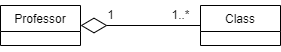
\includegraphics[width=4cm]{aggregation.png}
\end{center}
The professor has one or more classes to teach. A class has a professor.

\textbf{Composition}: Has a ``part of" relationship. When a container is destroyed, the contents are also destroyed.
\begin{center}
    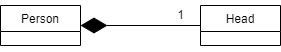
\includegraphics[width=4cm]{composition.png}
\end{center}
If person is deleted then head is also deleted as a result

\textbf{Generalization/Inheritance}: Has a ``is a" relationship. When a subclass is a specialized form of the other
\begin{center}
    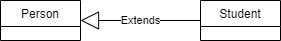
\includegraphics[width=4cm]{Generalization.png}
\end{center}

\textbf{Realization/Implementation}: A class implements the behavior that the interface specifies
\begin{center}
    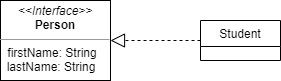
\includegraphics[width=4cm]{interface.png}
\end{center}
\vfill\null
\columnbreak
\textbf{UML Use Case Diagram}

Consider a system that deals with group tours. A tour guide has a task of group check-in, and that task involves a task of passenger check-in. When a passenger checks in, they may need to check in baggage. A passenger also has a task of being security screened, where they may need to submit to a full body scanner. A tour guide is also a passenger.

\begin{center}
    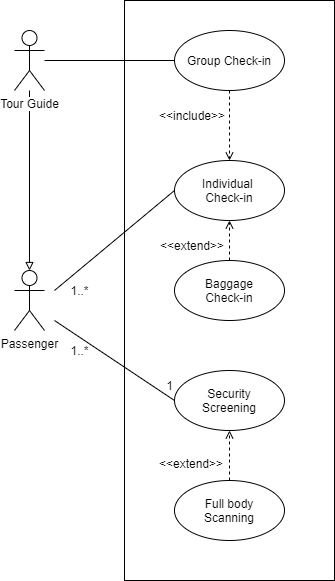
\includegraphics[width=4cm]{useCase.png}
\end{center}
\textbf{UML State Diagram}

Consider a simulator for an experiment. When triggered to run, the simulator begins running. The simulator can be paused and un-paused. Data can be requested from the simulator when it is paused. If there is data, it can be stored, showing a “data saved” message, after which the simulator must be explicitly triggered to continue running. If there is no data, a “no data” message is shown, and the simulator automatically continues running. Also, a running or paused simulator can be fully reset.
\begin{center}
    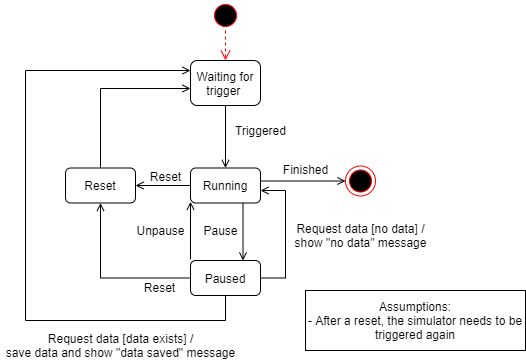
\includegraphics[width=6cm]{state.png}
\end{center}
\vfill\null
\columnbreak
\textbf{UML Sequence Diagram}

Consider the basic command design pattern, with Invoker, ConcreteCommand, and Receiver classes. Assume also there is a Client class to create a ConcreteCommand object and bind it to an Invoker object via dependency injection. Draw a complete and correct UML sequence diagram that depicts:
\begin{enumerate}
    \item the command creation and its binding to an invoker, and
    \item the behavior of the command pattern to have the invoker execute the command, which runs an action on a receiver
\end{enumerate}
\begin{center}
    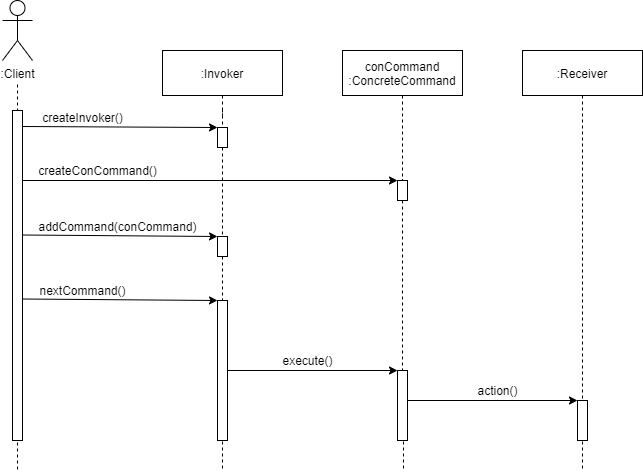
\includegraphics[width=6cm]{sequence.png}
\end{center}

\end{multicols*}
\newpage
\begin{multicols*}{2}
    \subsection*{Singleton Pattern}
    Intent: Ensure a class only has one instance and provide a global point of access to it
    \begin{lstlisting}
public class ExampleSingleton { // lazy construction
    private static ExampleSingleton instance = null;

    // protected constructor makes it possible to
    // create instances of subclasses
    protected ExampleSingleton() {
        ...
    }
    // lazy construction of the instance
    public static ExampleSingleton getInstance() {
        if (instance == null) {
            instance = new ExampleSingleton();
        }
        return instance;
    }
}
    \end{lstlisting}
    \subsection*{Composite Pattern}
    Intent: To compose individual objects to build up a tree structure (a folder can contains files and other folders). The individual objects and the composed objects are treated uniformly (files and folders both have a name)
    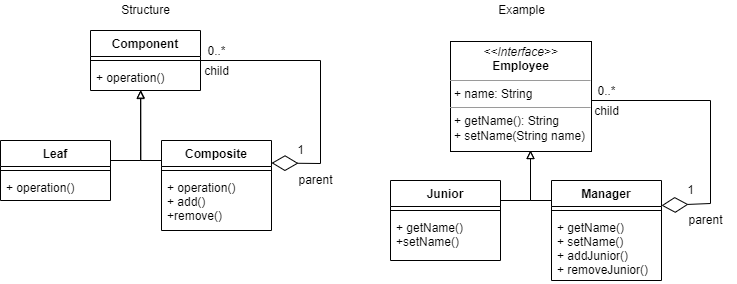
\includegraphics[width=10cm]{composite.png}

    \subsection*{Command Pattern}
    Intent: encapsulate a request as an object, so you can run, queue, log, undo/redo these requests. Also known as action/transaction. A class may want to issue a request without knowing anything about the operation being requested or the receiver object for the request

    \vfill\null
    \columnbreak

    \subsection*{Template Method Pattern}
    Intent: Define the skeleton of an algorithm in a method, deferring some steps to subclasses.
    Used when two classes share a lot of common methods. It reduces duplication and enhances reuse. \\
    \begin{center} 
        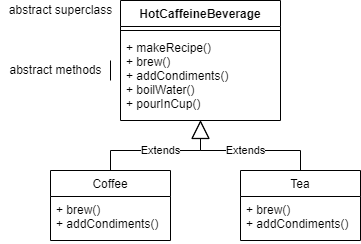
\includegraphics[width=6cm]{template.png}
    \end{center}

    \begin{lstlisting}
public abstract class HotCaffeineBeverage {
    // serves like a "template" for an algorithm,
    // where subclasses provide certain parts
    public final void makeRecipe() {
        boilWater();
        brew(); // from subclass
        pourInCup();
        addCondiments(); // from subclass
    }
    // let the subclasses determine how
    public abstract void brew();
    public abstract void addCondiments();
    public void boilWater() {
        System.out.println( "Boiling water" );
    }
    public void pourInCup() {
        System.out.println( "Pouring into cup" );
    }
}           
    \end{lstlisting}

    \begin{lstlisting}
// subclasses inherit
// makeRecipe, boilWater, pourInCup
public class Coffee extends HotCaffeineBeverage {
    public void brew() {
        System.out.println( "Brewing the coffee" );
    }
    public void addCondiments() {
        System.out.println( "Adding sugar, milk" );
    }
}
public class Tea extends HotCaffeineBeverage {
    public void brew() {
        System.out.println( "Steeping the tea" );
        System.out.println( "Removing the tea" );
    }
    public void addCondiments() {
        System.out.println( "Adding lemon" );
    }
}
                
    \end{lstlisting}

\end{multicols*}
\newpage
\begin{multicols*}{2}
    \subsection*{Factory Method Pattern}
    Intent: Define an interface for creating an object, but lets subclasses decide which actual class to instantiate.
    \begin{center} 
        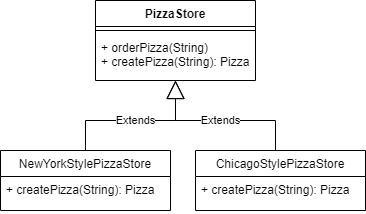
\includegraphics[width=6cm]{factory.png}
    \end{center}

    \begin{lstlisting}
public abstract class PizzaStore {
    public Pizza orderPizza( String pizzaType ) {
        Pizza pizza;
        pizza = createPizza( pizzaType );
        
        pizza.bake();
        pizza.cut();
        pizza.box();
        return pizza;
    }
    // defer to subclass to instantiate
    // Pizza of the appropriate type
    public abstract Pizza createPizza(String pizzaType);
}               
    \end{lstlisting}
    \begin{lstlisting}
public class NewYorkStylePizzaStore extends PizzaStore {
    public Pizza createPizza( String pizzaType ) {
        if (pizzaType.equals( "pepperoni" ) {
            Pizza pizza =
            new NewYorkStylePepperoniPizza();
        } else if (pizzaType.equals( "veggie" ) {
            Pizza pizza =
            new NewYorkStyleVeggiePizza();
        }
        return pizza;
    }
}        
    \end{lstlisting}
    \subsection*{Adapter Pattern}
    Intent: convert the interface of a class into another interface that clients expect. This lets classes work together that couldn't otherwise because of incompatible interfaces. Also known as a wrapper.

    \begin{center} 
        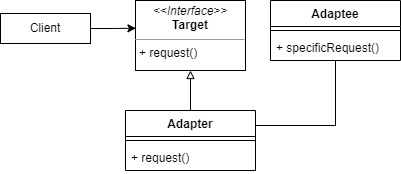
\includegraphics[width=8cm]{wrapper.png}
    \end{center}

    \begin{lstlisting}
// target interface
public interface Duck {
    public void fly();
    public void quack();
} 
    \end{lstlisting}
    \begin{lstlisting}
// adaptee
public class Turkey {
    public void fly() { ... }
    public void gobble() { ... }
}
    \end{lstlisting}
    \begin{lstlisting}
// adapter
public class TurkeyAdapter implements Duck {
    Turkey turkey;
    public TurkeyAdapter( Turkey turkey ) {
        this.turkey = turkey;
    }
    public void fly() {
        for (int i = 0; i < 5; i++) turkey.fly();
    }
    public void quack() {
        turkey.gobble();
    }
}
    \end{lstlisting}
    \subsection*{Proxy Pattern}
    Intent: to provide a surrogate or placeholder for another object to control access to it. It is used to defer the full cost of creation and initialization of an object until we actually need to use it
    \begin{center} 
        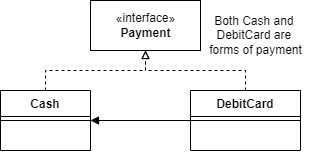
\includegraphics[width=6cm]{proxy.png}
    \end{center}

    \newpage
    \subsection*{State Pattern}
    Intent: allow an object to alter its behavior when its internal state changes. To code a state model.
    For example, a simple pop machine where you can insert a loonie, press dispense button, and get a pop. We could eject to return money and the machine has a limited supply. The state diagram is the following:
    \begin{center} 
        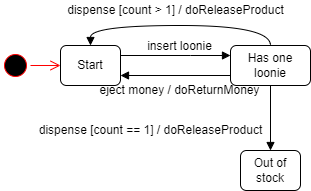
\includegraphics[width=6cm]{proxystate.png}
        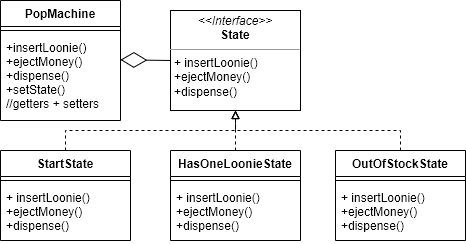
\includegraphics[width=8cm]{stateUML.png}
    \end{center}
    \begin{lstlisting}
// common interface for pop machine state classes
interface State {
    // all potential triggers
    public void insertLoonie( PopMachine popMachine );
    public void ejectMoney( PopMachine popMachine );
    public void dispense( PopMachine popMachine );
}
    \end{lstlisting}
    \begin{lstlisting}
class StartState implements State {
    public void insertLoonie( PopMachine popMachine ) {
        System.out.println( "loonie inserted" );
        popMachine.setState(
        popMachine.getHasOneLoonieState());
    }
    public void ejectMoney( PopMachine popMachine ) {
        System.out.println( "no money to return" );
    }
    public void dispense( PopMachine popMachine ) {
        System.out.println( "payment required" );
    }
}           
    \end{lstlisting}
    \begin{lstlisting}
class HasOneLoonieState implements State {
    public void insertLoonie( PopMachine popMachine ) {
        System.out.println( "already have one loonie" );
    }
    public void ejectMoney( PopMachine popMachine ) {
        System.out.println( "returning money" );
        popMachine.doReturnMoney();
        popMachine.setState(
        popMachine.getStartState());      
    } 
    public void dispense( PopMachine popMachine ) {
        System.out.println( "releasing product" );
        popMachine.doReleaseProduct();
        if (popMachine.getCount() > 0) {
            popMachine.setState(
            popMachine.getStartState());
        } else {
            popMachine.setState(
            popMachine.getOutOfStockState());
        }
    }
}                   
    \end{lstlisting}
    \begin{lstlisting}
class OutOfStockState implements State {
    public void insertLoonie( PopMachine popMachine ) {
        System.out.println( "machine out of stock" );
    }
    public void ejectMoney( PopMachine popMachine ) {
        System.out.println( "no money to return" );
    }
    public void dispense( PopMachine popMachine ) {
        System.out.println( "machine out of stock" );
    }
}                             
    \end{lstlisting}
    \begin{lstlisting}
public class PopMachine {
    private State startState;
    private State hasOneLoonieState;
    private State outOfStockState;
    private State currentState;
    private int count;
    public PopMachine( int count ) {
        // make the needed states
        startState = new StartState();
        hasOneLoonieState = new HasOneLoonieState();
        outOfStockState = new OutOfStockState();
        if (count > 0) {
            currentState = startState;
            this.count = count;
        } else {
            currentState = outOfStockState;
            this.count = 0;
        }
    } 
    public void insertLoonie() {
        currentState.insertLoonie( this );
    }
    public void ejectMoney() {
        currentState.ejectMoney( this );
    }
    public void dispense() {
        currentState.dispense( this );
    }
    public void setState( State state ) {
        currentState = state;
    }
    public int getCount() {
        return count;
    }
    // getters for state objects, machine actions, etc.
}
                                       
    \end{lstlisting}
    \newpage
    \subsection*{Decorator pattern}
    Intent: attach additional responsibilities to an object dynamically. It is usually used for making user interface embellishments such as adding decorations like a menu bar, vertical scrollbar, or horizontal scrollbar to a basic window. It's used when you don't want too many new subclasses. You use aggregation instead of inheritance

    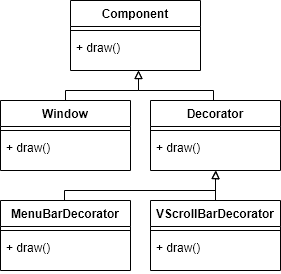
\includegraphics[width=6cm]{decorator.png}

    \subsection*{Chain of responsibility pattern}
    Intent: avoid coupling the sender of a request to its receiver by giving more than one object a chance to handle the request. Chain the receiving objects and pass the request along the chain until an object handles it.
    \begin{center} 
        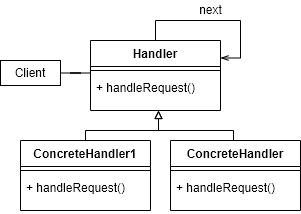
\includegraphics[width=8cm]{respons.png}
    \end{center}
    Example:
    \begin{center} 
        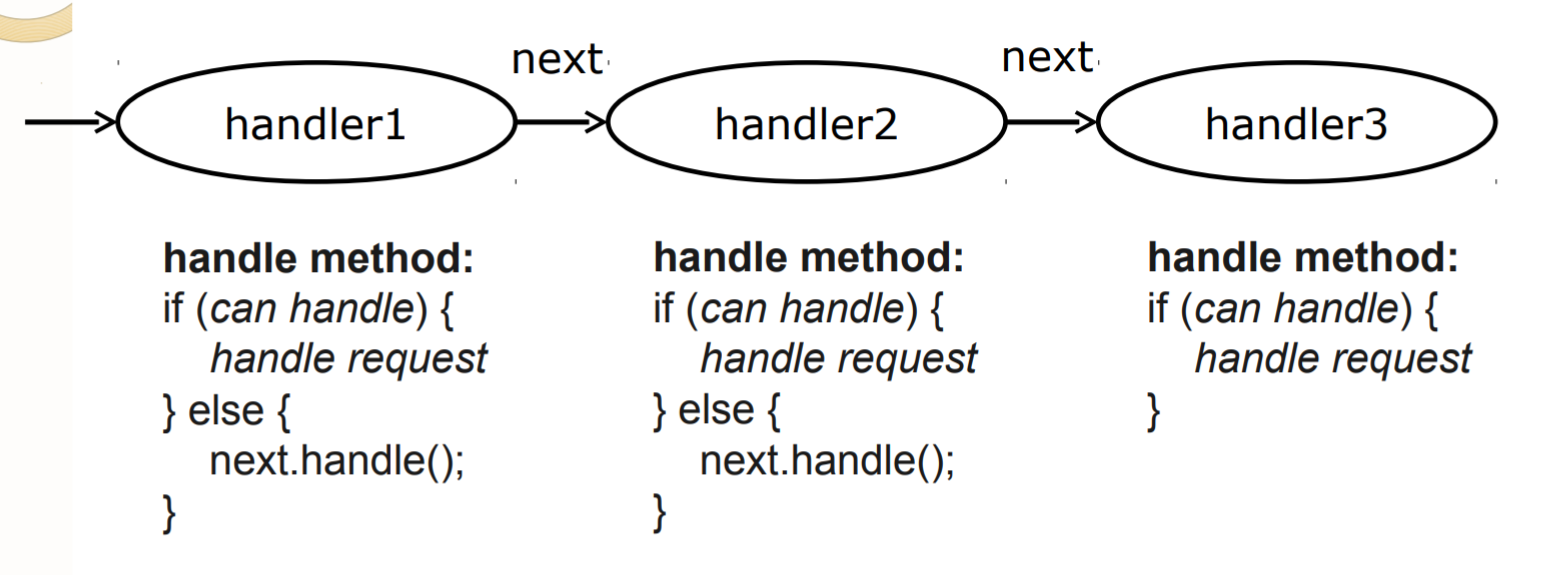
\includegraphics[width=8cm]{handler.png}
    \end{center}

    \subsection*{Design Principles}
    The goals is to enhance flexibility under changing needs and improve reusability in different contexts. \\\\
    \textbf{Open closed principle}: Classes should be open for extension but closed for modification. Feel free to extend the classes and add new classes when needing changes. Existing classes are tested and work so do not tinker with them. ``Encapsulate what varies'' \\\\
    \textbf{Dependency inversion principle}: Depend upon abstractions. Do not depend on concrete classes. Program to interfaces, not implementations. Favor composing objects over implementation inheritance. \\\\
    \textbf{Principle of least knowledge}: ``Only talk to your immediate friends.'' For an object, reduce the number of classes it knows about and interacts with. Reduces coupling and changes cascading throughout the system.

    Law of demeter:
    Avoid calling methods of objects returned by other methods. ``One dot only rule''
    For method M of object O, only call methods of the following objects:
    \begin{enumerate}
        \item Object O itself
        \item parameters of method M
        \item any objects instantiated within method M
        \item direct component objects of object O
    \end{enumerate}
\end{multicols*}

\end{document}